\chapter{Proposta de pesquisa}
\label{capitulo:proposta}

\section{Tema}

As redes neurais artificiais (RNA) compõem um novo paradigma para geração de dados sintéticos como as \textit{generative adversarial networks} (GANs). Esses modelos computacionais têm a capacidade de produzir conjuntos de dados sintéticos a partir de imagens, séries temporais e dados tabulares, que podem conter diversos tipos de variáveis sejam elas contínuas, discretas ou categóricas. Apesar de já existirem técnicas estatísticas para geração de dados sintéticos como aquelas baseadas em redes bayesianas, as GANs têm se destacado devido aos seus resultados, que demonstram melhores métricas de similaridade estatística e eficácia de aprendizado de máquina \cite{xu2019}.

Trabalhos mais recentes na área de pesquisa da geração de dados sintéticos têm proposto novas técnicas, como os modelos de difusão estável, capazes de alcançar desempenhos superiores às GANs em termos de eficácia de aprendizado de máquina, como observado em \citeonline{diffusion-beats-gan}.

O principal desafio desses modelos é assegurar um bom equilíbrio entre utilidade estatística e privacidade como observado em \citeonline{wang2021}. A principal aplicação envolve a utilização de conjuntos de dados sintéticos para o desenvolvimento de análises estatísticas e modelos computacionais, mas com garantias de que os dados reais estejam protegidos, por exemplo, contra \textit{Linkage Attacks}, técnica na qual tenta-se inferir atributos sensíveis de observações reais a partir de modelos computacionais treinados com dados sintéticos.

\section{Motivação}

Os dados são um insumo fundamental para o desenvolvimento da pesquisa científica e da tecnologia na indústria. Neste contexto, os modelos generativos para a construção de conjuntos de dados sintéticos são potenciais catalisadores de inovação, uma vez que possibilitam a exploração e construção de novas tecnologias que exigem dados sensíveis para seu desenvolvimento, como aplicações nas áreas de finanças, saúde, microscopia e sensoriamento remoto\cite{review2022}.

Além disso, é notável que o desenvolvimento de algoritmos eficientes para geração de dados sintéticos podem contribuir para a construção de modelos mais sofisticados utilizando técnicas de \textit{deep learning}.

Sob a óptica científica, além de se beneficiar do acesso a mais informações, há também um ganho na reprodutibilidade dos experimentos, já que mais conjuntos de dados podem ser compartilhados junto aos resultados experimentais das análises, mesmo aqueles que possuam características sensíveis.


\section{Lacuna}

Apesar dos resultados promissores dos modelos generativos em termos de desempenho de aprendizagem de máquina, a literatura atual carece de métodos de avaliação que explorem a explicabilidade dos modelos propostos. Esta lacuna pode comprometer a seleção de modelos baseados em dados sintéticos, pois não investiga a multiplicidade de bons modelos que podem levar ao efeito \textit{Rashomon}, em que diferentes modelos apresentam o mesmo desempenho, mas aprendem características distintas, levando a problemas de generalização por sub-espeficicação como já observado em \citeonline{breimanStatisticalModeling2001} e \citeonline{underspecification}.

\section{Questão de pesquisa}

Dado o contexto introduzido, este trabalho tem por objetivo responder a seguinte questão de pesquisa: Modelos de classificação baseados em \textit{deep learning}, treinados em conjuntos de imagens reais e sintéticas, possuem desempenho similares em conjuntos de testes independentes e identicamente distribuídos (i.i.d.) e aprendem os mesmos padrões para a resolução do problema?

Esta questão de pesquisa será respondida por meio da proposição e validação de um método abrangente de avaliação que permita avaliar os modelos em conjuntos de teste i.i.d. e aplicar outras medidas de explicabilidade que possibilitem a compreensão das relações aprendidas pelos modelos submetidos ao método.

Espera-se que o método proposto seja capaz de avaliar a capacidade de generalização dos modelo, contribuindo também para um melhor entendimento das características relevantes identificadas pelos modelos para a solução dos problemas.

\subsection{Justificativa}

A resposta para a questão de pesquisa deste trabalho contribui para um avanço no estabelecimento de um \textit{common task framework}\cite{ctf} mais robusto que possibilita identificar falhas de generalização e especificação em modelos de \textit{deep learning} treinados em imagens sintetizadas. Deste modo, ao estabelecer um método mais abrangente de avaliação, ganha-se riqueza na interpretação da performance e explicabilidade do modelo, adicionando informações que servem como guia para trabalhos futuros de melhorias nos modelos de geração de imagens já existentes e também no desenvolvimento de classificadores baseados em redes neurais.

\section{Objetivo}

O objetivo deste trabalho é propor e desenvolver um arcabouço para avaliação do desempenho de modelos de \textit{deep learning} na tarefa de classificação de imagens, treinados em conjuntos de dados sintéticos e reais, levando em consideração métricas e conjuntos de dados padronizados, possibilitando que modelos treinados com conjuntos de dados reais e sintéticos - provenientes de diferentes modelos de geração de imagens - possam ser avaliados sob a luz de métricas que possibilitem a detecção de falhas de generalização e especificação.

\section{Metodologia}
\label{secao:metodologia}

Este trabalho se concentra na área de explicabilidade de modelos de aprendizagem de máquina construídos a partir de imagens sintéticas geradas por \textit{generative adversarial networks} (GANs) e \textit{diffusion models}. Por meio de técnicas padrão-ouro de avaliação de modelos de classificação e métodos de explicabilidade aplicados a modelos de classificação de imagens, será proposto e implementado uma suíte de avaliação robusta e abrangente. Com base na revisão bibliográfica, diferentes modelos de geração de imagens sintéticas serão selecionados e implementados para a geração de conjuntos de imagens sintéticas a partir de conjuntos de dados pré definidos, assim, modelos de classificação com performance estado-da-arte serão treinados e avaliados pelo arcabouço proposto neste trabalho em diferentes cenários de composições de conjuntos de dados com imagens reais e sintéticas.

\begin{enumerate}

    \item \label{a0} \textbf{Redação da dissertação}: escrita dos componentes textuais da dissertação.

    \item \label{a1} \textbf{Seleção e implementação dos modelos de geração de imagens}: por meio dos dados levantados na revisão sistemática definiremos os modelos a serem implementados utilizando a linguagem Python.
    
    \item \label{a2} \textbf{Coleta de conjuntos de dados}: serão selecionados e coletados conjuntos de dados com diferentes características como número de classes representadas e balanceamentos de classes para a avaliação dos resultados em diferentes cenários de treinamentos.
    
    \item \label{a3} \textbf{Geração dos conjuntos de imagens sintéticas}: A partir dos modelos de geração implementados serão gerados novos conjuntos de dados com imagens sintéticas.
    
    \item \label{a4} \textbf{Seleção e implementação dos modelos classificadores}: Implementação e treinamento dos modelos de classificação em conjuntos de dados com diferentes proporções de imagens geradas sinteticamente. 

    \item \label{a5} \textbf{Proposta e implementação do framework de avaliação}: Definição e implementação de métricas padrão-ouro na literatura para avaliação de modelos de classificação e interpretabilidade.
    
    \item \label{a6} \textbf{Aplicação do framework}: Submissão dos resultados dos modelos ao framework de avaliação.
    
    \item \label{a7} \textbf{Avaliação dos resultados}: Discussão em detalhes dos resultados obtidos na atividade \ref{a6}.
    
    \item \label{a8} \textbf{Divulgação}: Submissão de artigo para revista da área.
\end{enumerate}

\subsection{Cronograma}

Além das atividades programadas com base na metodologia proposta, durante a revisão de literatura um estudo piloto foi conduzido para avaliar a aplicabilidade e viabilidade do arcabouço de avaliação proposto. O capítulo 
\ref{capitulo:estudo-piloto} trás mais detalhes sobre o estudo piloto, enquanto a seção \ref{secao:arcabouco} explica em mais detalhes o arcabouço de avaliação. O quadro \ref{quadro:cronograma} apresenta a organização cronológica das atividades propostas na seção \ref{secao:metodologia}.

\hskip-1.2cm
\begin{quadro}[h]
    \caption{Cronograma do projeto.}
    \centering
    \resizebox{\textwidth}{!}{
    % {p{2in} p{3in} p{3in} p{2in} p{1in} p{2in}
    \begin{tabular}{|p{0.5in}|p{3in}|c|c|c|c|c|c|c|}
        \hline
            \multicolumn{2}{|c|}{Atividade} &
            \multicolumn{2}{|c|}{2023} &
            \multicolumn{4}{|c|}{2024}
            \\
        \hline
            Num. &
            Descrição &
            1 Sem &
            2 Sem &
            1 Tri &
            2 Tri &
            3 Tri &
            4 Tri \\
        \hline
            0 &
            Revisão Bibliográfica &
            X&X&X&X&& \\ 
        \hline
            0.1 &
            Estudo Piloto &
            &X&X&&& \\ 
        \hline
            \ref{a0} &
            Redação da Dissertação &
            X&X&X&X&X&X \\ 
        \hline
            \ref{a1} &
            Implementação dos modelos de geração de imagens &
            &&&X&& \\
        \hline
            \ref{a2} &
            Coleta de conjuntos de dados &
            &&&X&& \\
        \hline
            \ref{a3} &
            Geração dos conjuntos de imagens sintéticas &
            &&&X&& \\
        \hline
            \ref{a4} &
            Implementação dos modelos classificadores &
            &&&&X& \\
        \hline
            \ref{a5} &
            Proposta e implementação do \textit{framework} de avaliação &
            &&&&X& \\
        \hline
            \ref{a6} &
            Aplicação do \textit{framework} &
            &&&&X& \\
        \hline
            \ref{a7} &
            Avaliação dos resultados &
            &&&&&X \\
        \hline
            \ref{a8} &
            Divulgação &
            &&&&&X \\
        \hline
    \end{tabular}
    }
    \label{quadro:cronograma}
    \source{Alexandre Farias, 2024}
\end{quadro}


\subsection{Arcabouço Proposto} \label{secao:arcabouco}

A figura \ref{fig:arcabouco-proposto} esquematiza de forma simples a metodologia proposta para a avaliação da questão de pesquisa definida neste trabalho.
A partir de um banco de imagens definido previamente, dois conjuntos de dados serão derivados sendo o conjunto de treinamento e um conjunto de teste. O conjunto de treinamento real será utilizado para treinar os modelos geradores de imagens sintéticas e assim produzir um segundo conjunto de dados de treinamento sintético, além disso, também será empregado para o treinamento dos classificadores. Por fim, os conjuntos de dados de testes serão compostos apenas por imagens reais, que serão avaliadas pelos modelos classificadores.

\begin{figure}[htbp]
	\centering
	\caption[Esquema da metodologia proposta para avaliação da hipótese]{Esquema da metodologia proposta para avaliação da hipótese: mantendo o modelo padrão de avaliação de eficácia de aprendizado de máquina aplicado a modelos de classificação, o arcabouço proposto adiciona uma nova camada de interpretabilidade para ajudar a validar com mais rigor a hipótese de utilidade dos dados sintéticos.}
		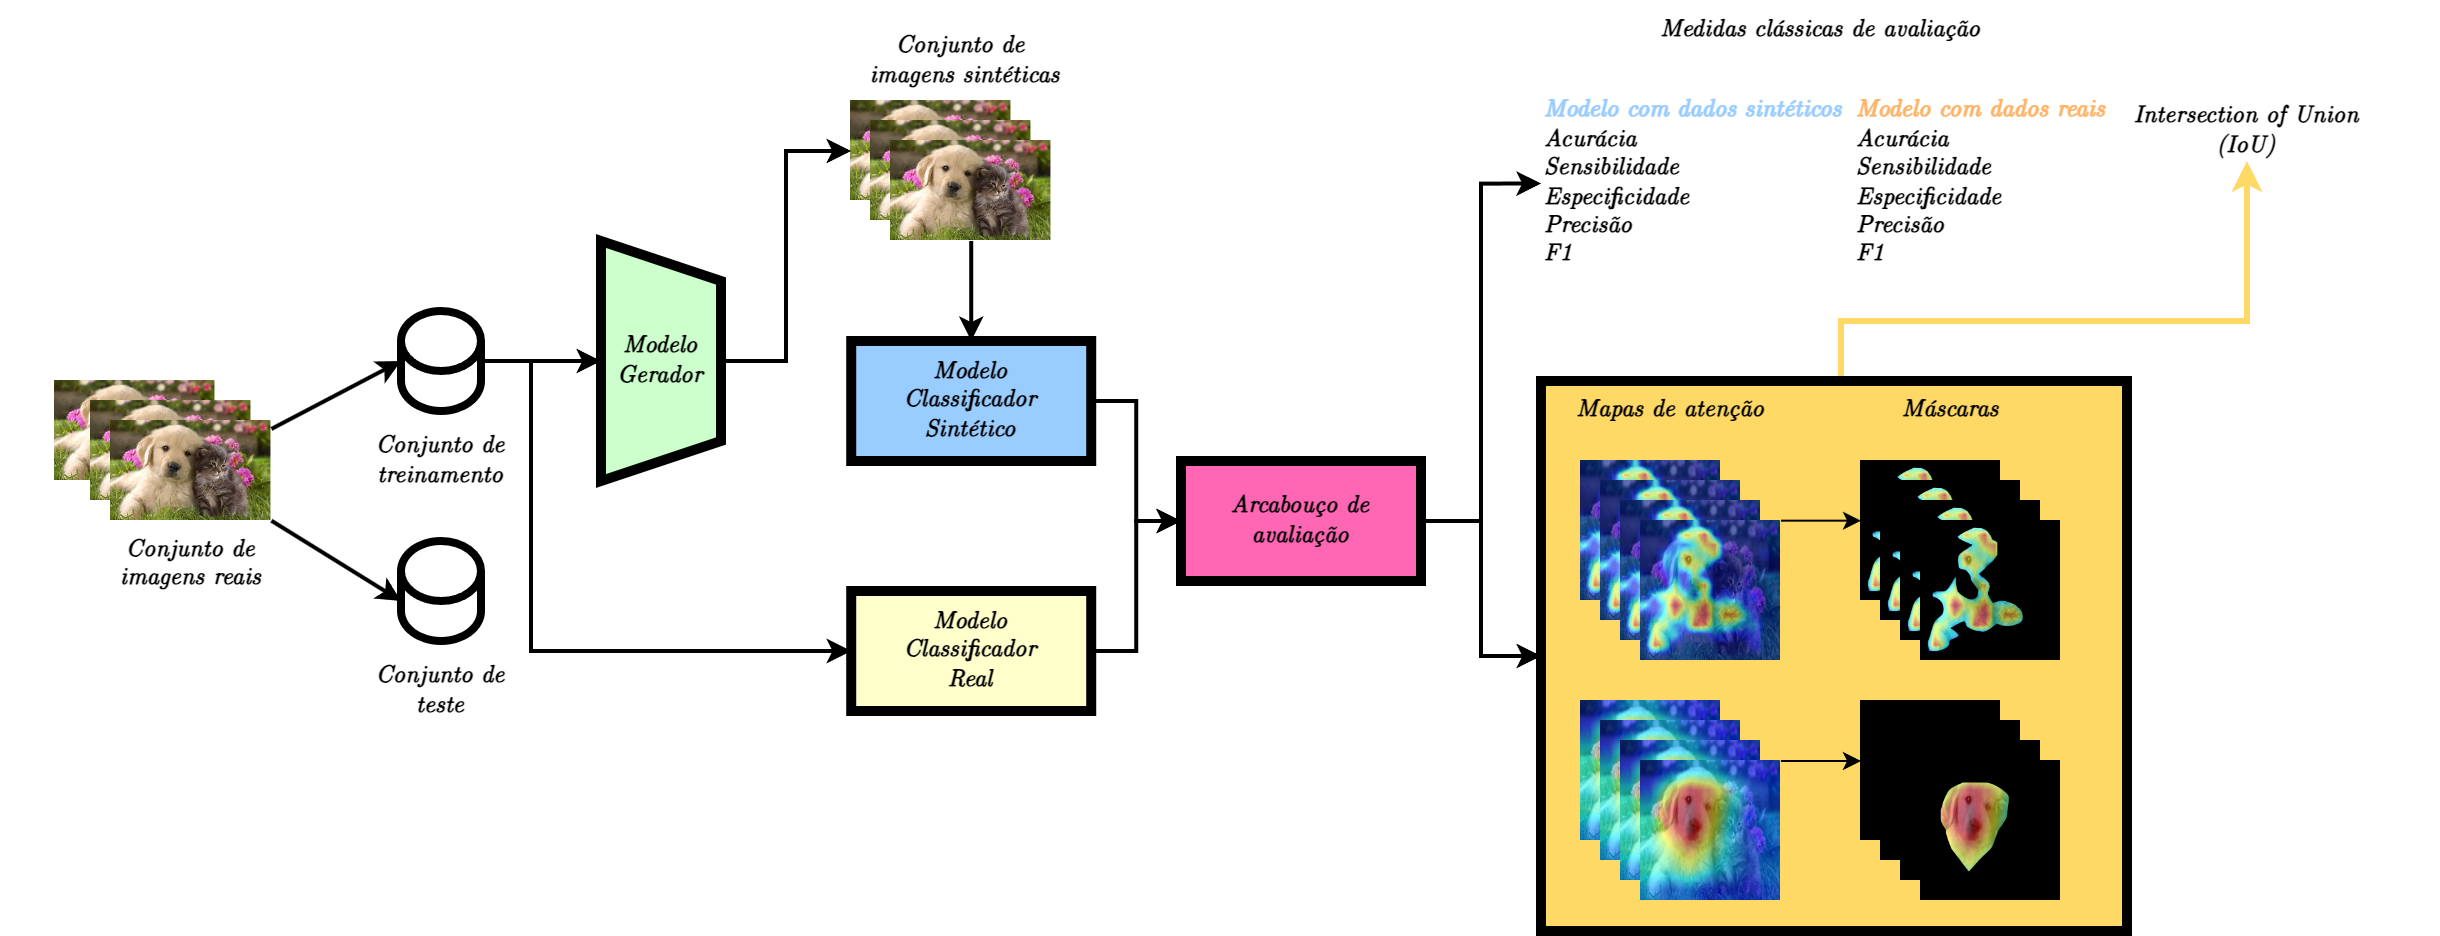
\includegraphics[scale=.19]{imagens/arcabouco-proposto.png}
	\label{fig:arcabouco-proposto}
  \source{Alexandre Farias, 2024}
\end{figure}

Os modelos classificadores serão treinados ao menos em dois cenários específicos, no primeiro cenário (a) considerando apenas imagens reais e no segundo cenário (b) considerando apenas imagens sintéticas. Na etapa de treinamento, um conjunto de validação será derivado do respectivo conjunto de treinamento para evitar o sobre-ajuste dos modelos e definir critérios de parada antecipada.

\subsubsection{Avaliação}

Utilizando o conjunto de teste os modelos serão submetidos a uma avaliação clássica utilizando as principais métricas encontradas na literatura, como acurácia, precisão, sensibilidade, especificidade e F1.

Juntamente da avaliação de eficácia de aprendizado de máquina, mapas de atenção serão gerados para ambos os modelos em todas as imagens do conjunto de testes utilizando a técnica Grad-CAM++. Com base nos mapas de atenção, técnicas de processamento de imagens serão utilizadas para produzir máscaras que serão posteriormente empregadas para o cálculo da métrica \textit{Intersection of Union} (IoU) que auxiliará na avaliação da similaridade das características aprendidas pelos diferentes modelos.

\subsubsection{Conjuntos de dados}

Para aplicar a metodologia proposta serão utilizados os conjuntos de dados \textit{Chest X-Ray Images (Pneumonia)} utilizado em \citeonline{xraychestdataset} e CIFAR-10\footnote{https://www.cs.toronto.edu/~kriz/cifar.html}. O Primeiro conjunto de dados contem imagens de raio-x de tórax de pulmões saudáveis e não saudáveis, o problema de aprendizado a ser resolvido será a classificação binária. Já o segundo conjunto de dados, contêm imagens de várias classes distintas, como aviões, automóveis, cães, gatos, navios e outros animais, para este conjunto de dados o objetivo será o desenvolvimento de um classificador multi-classe.
Além da notável diferença na natureza dos conjuntos de dados, a escolha dos conjuntos se dá também pela diferença de diversidade das amostras, permitindo avaliar os modelos de geração e classificação em conjuntos de menor e maior nível de variação entre as instâncias.

\section{Contribuições}
O desenvolvimento deste projeto contribui para o avanço na metodologia de desenvolvimento e avaliação de modelos de geração de imagens e modelos de classificação treinados em conjuntos de dados sintéticos. Especificamente serão produtos deste trabalho:

\begin{enumerate}
    \item Método de avaliação padronizado contemplando o padrão-ouro atual e novas medidas de interpretabilidade relevantes para detectar problemas de sub-especificação.
    \item Biblioteca \textit{open source} na linguagem de programação Python com o método proposto implementado.
\end{enumerate}


\section{Escopo}

O escopo desta pesquisa se limita a avaliação de modelos de classificação treinados em conjuntos de imagens sintéticas geradas por GANs e \textit{diffusion models}. O presente projeto não inclui a avaliação da qualidade de séries temporais, conjuntos de dados relacionais ou dados tabulares sintéticos. Os métodos de geração e avaliação envolvidos neste trabalho não se aplicam a dados tabulares estruturados.
